\documentclass[t]{beamer}
\usepackage{beamerthemesplit}
\usepackage{xcolor}
\usepackage{color}
\usepackage{colortbl}
\usepackage{tikz}
\usepackage{epsfig}
\usepackage{epstopdf}
\usepackage{subfigure}
\usepackage[absolute,overlay]{textpos}
\usetheme{USC}

\tikzset{
  every overlay node/.style={
    draw=none,fill=none,rounded corners,anchor=north west,
  },
}
% Usage:
% \tikzoverlay at (-1cm,-5cm) {content};
% or
% \tikzoverlay[text width=5cm] at (-1cm,-5cm) {content};
\def\tikzoverlay{%
   \tikz[baseline,overlay]\node[every overlay node]
}%

\definecolor{mygreen}{RGB}{0, 108, 57}

\usepackage{amsmath}
\usepackage{mathtools}
\DeclareMathOperator*{\argmax}{arg\,max}

% Table
\usepackage{multirow}
\usepackage{colortbl}
\definecolor{kugray5}{RGB}{224,224,224}
\usepackage{rotating}

\begin{document}

\graphicspath{ {Graphics/}{Graphics/old/} }

\title[USC Viterbi School of Engineering]{An On-line Truthful and Individually Rational Pricing Mechanism for Ride-sharing}  
\author[Mohammad Asghari]{\small{Speaker:}\\Mohammad Asghari\\
\vspace{0.05in}
\begin{flushleft}
\tiny{
\hspace{1.25in}Joint work with\\
\hspace{1.25in}Cyrus Shahabi, Faculty of CS Department at USC}\\
\vspace{-0.25in}
\end{flushleft}}

\date{Nov 8, 2017} 
\begin{frame}
\titlepage
\vspace{-0.5in}
\begin{columns}
  \column{.2\textwidth}
  \begin{center}
    
\includegraphics[height=1.5cm]{viterbi_logo.jpg}
  \end{center}
  \column{.6\textwidth}
  \column{.2\textwidth}
  \begin{center}
    
\includegraphics[height=1.5cm]{imsc_logo.jpg}   
  \end{center}
\end{columns} 
\end{frame}

\section*{Introduction}
\begin{frame}\frametitle{Motivation}
\begin{figure}
	\centering
    
\includegraphics[width = 0.75\columnwidth]{carpool.eps}
\end{figure}
\begin{itemize}
\item<2-> Increasing popularity of commercial ride-sharing platforms
\begin{figure}
	\centering
    
\includegraphics[width = 0.55\columnwidth]{ride-sharings.eps}
\end{figure}
\end{itemize}
\end{frame}

\begin{frame}\frametitle{Motivation}
\vspace{-0.28in}
\begin{figure}
	\centering
    
\includegraphics[width = 0.55\columnwidth]{ride-sharings.eps}
\end{figure}
\vspace{-0.23in}
\begin{itemize}
\item Monetary Incentives.
\item<2-> Price-aware Real-time Ride-sharing at Scale \textbf{(SIGSPATIAL'16) [1]} 
\vspace{-0.1in}
\only<3->{
\begin{figure}
	\centering
    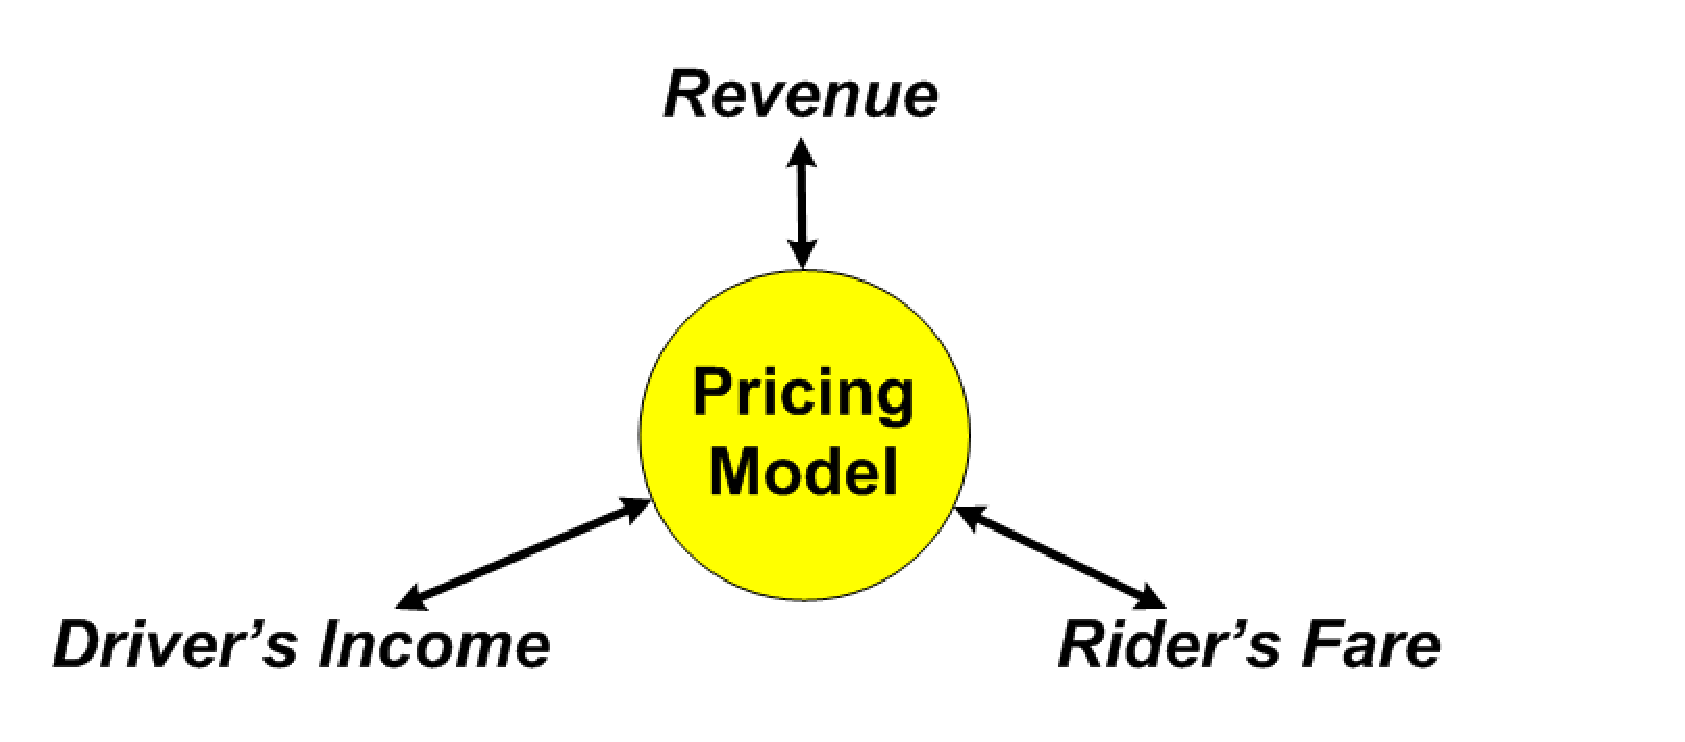
\includegraphics[width = 0.75\columnwidth]{pricing3.eps}
\end{figure}
}
\end{itemize}
\only<3->{
\vspace{0.2in}
\tiny{[1] Asghari et. al., Price-aware Real-time Ride-sharing at Scale - An Auction-based Approach, SIGSPATIAL'16, San Francisco, CA}
}
\only<4>{
\begin{textblock*}{7cm}(3cm,4.5cm)
\begin{block}{}
\begin{itemize}
\item \large{\textbf{Can the drivers cheat?}}
\item \large{\textbf{How can we prevent it without sacrificing revenue?}}
\end{itemize}

\end{block}
\end{textblock*}
}
\end{frame}

\section{Framework Overview}
\frame{\frametitle{Outline}\tableofcontents}

\begin{frame}\frametitle{Rider's Fare}
for every request \textit{r}:
\begin{itemize}
\item<1-> $\phi_r$: shortest path between $r.s$ and $r.e$
\item<2-> $F: \mathbb{R}_{+}  \rightarrow \$ $ such that $F(\phi_r)$ is the default fare of a ride
\end{itemize}
\begin{columns}
\column{0.5\textwidth}
\begin{itemize}
\item<3-> $\hat{\phi}_r$: actual trip of \textit{r}
\item<3-> $\Delta_r = \frac{\hat{\phi}_r - \phi_r}{\phi_r}$
\item<4-> $\lambda: \mathbb{R}_{+} \rightarrow \left[ 0, 1 \right] $ specifies the discount for $\Delta_r \in \mathbb{R}_{+}$
\end{itemize}
\vspace{0.25in}
\only<5->{
\begin{block}{}
\begin{equation*}
fare(r) = F(\phi_r) \cdot \lambda(\Delta_r)
\end{equation*}
\end{block}
}

\column{0.5\textwidth}
\only<5->{
\begin{center}
\footnotesize{Rider Profile Example}
\end{center}
\vspace{-0.15in}
\begin{figure}
	\centering
    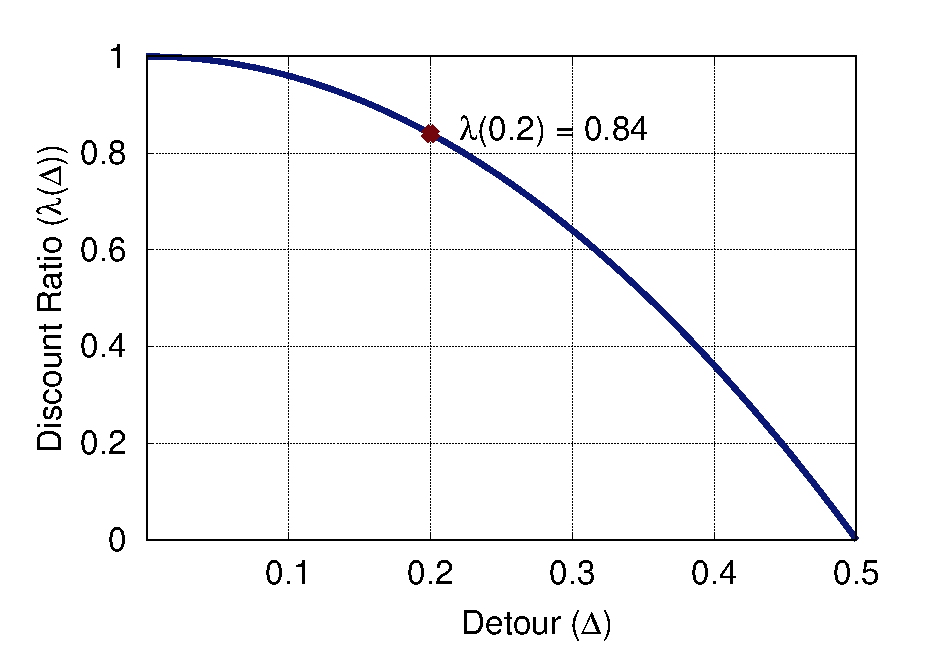
\includegraphics[width = 0.95\columnwidth]{rider_profile}
    \label{fig:quality}
\end{figure}
}
\end{columns}
\end{frame}

\begin{frame}\frametitle{Driver's Cost}
\vspace{-0.15in}
for every driver \textit{v}:
\begin{itemize}
\item $\theta: \mathbb{R}_{+}  \rightarrow \$ $ specifies the monetary cost of \textit{v} driving a distance $d \in \mathbb{R}_{+}$
\begin{itemize}
\item<2-> $\theta: \mathbb{N} \times \mathbb{R}_{+}  \rightarrow \$$
\end{itemize}
\end{itemize}
\begin{columns}
\column{0.60\textwidth}
\vspace{-0.1in}
\only<4->{
\begin{exampleblock}{}
\begin{equation*}
cost(\pi_d, \hat{\theta_d}) = \int_{start_{\pi_d}}^{end_{\pi_d}} \mathbb{I}\left\lbrace \pi_d^t \neq \left\langle \right\rangle\right\rbrace.\hat{\theta_d}(t)dt
\end{equation*}
\begin{itemize}
\item $\mathbb{I}$: indicator function
\item $\pi_d^t$: driver's schedule at \textit{t}. 
\item $start_{\pi_d}$: first pick-up time of $\pi_d$
\item $end_{\pi_d}$: last drop-off time of $\pi_d$
\end{itemize}
\end{exampleblock}
}
\column{0.40\textwidth}
\only<3->{
\begin{center}
\footnotesize{Driver Profile Example}
\end{center}
\vspace{-0.15in}
\begin{figure}
	\centering
    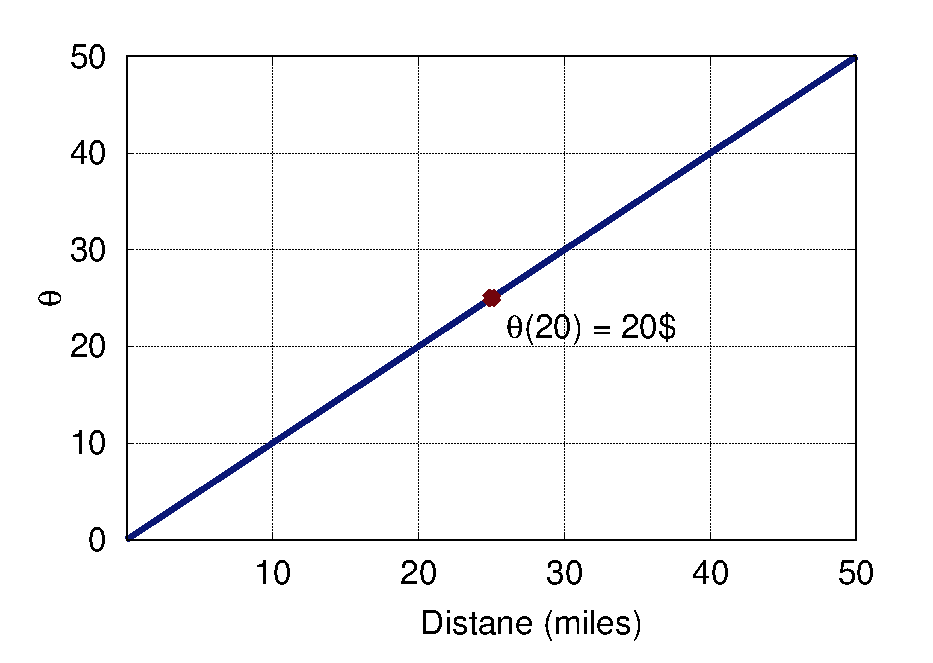
\includegraphics[width = 0.95\columnwidth]{driver_profile}
    \label{fig:quality}
\end{figure}
}
\end{columns}
\end{frame}

\begin{frame}\frametitle{Task Dispatching}
\only<1>{
\vspace{-0.15in}
\begin{figure}
	\centering
    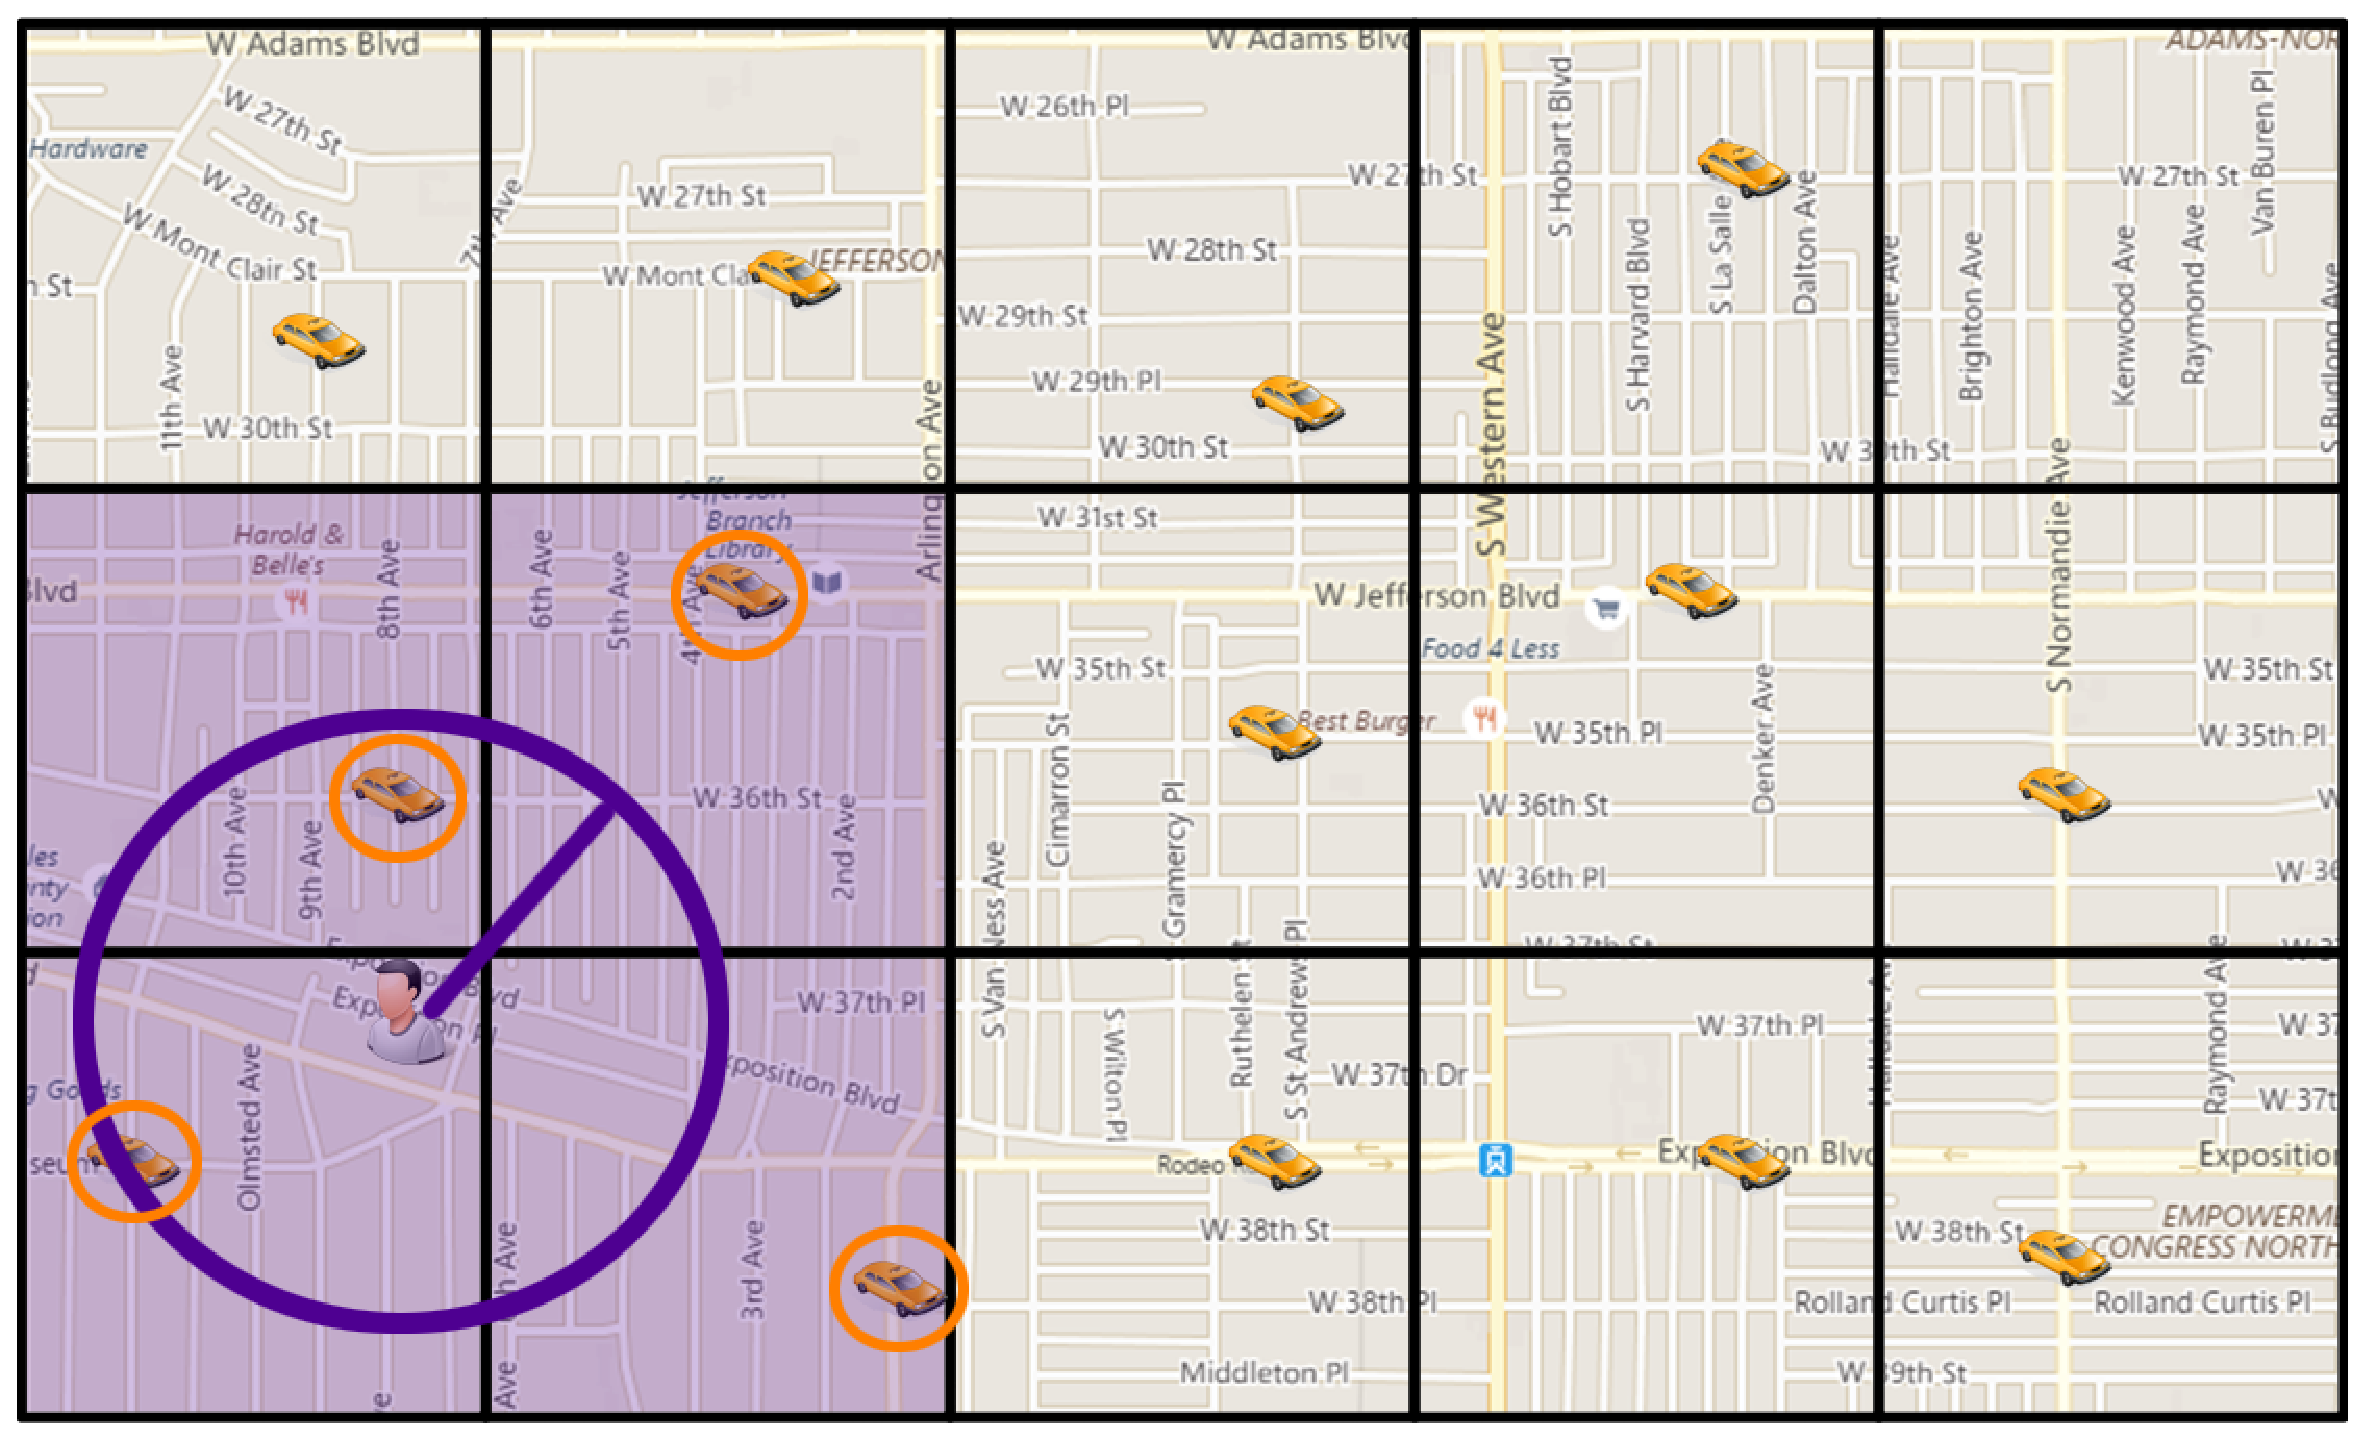
\includegraphics[width = 0.95\columnwidth]{rs_dispatch}
\end{figure}
}
\end{frame}

\begin{frame}\frametitle{Bid Computation}
\begin{columns}
\column{0.7\textwidth}
\vspace{-0.3in}
\only<1>{
\vspace{-0.15in}
\begin{figure}
	\centering
    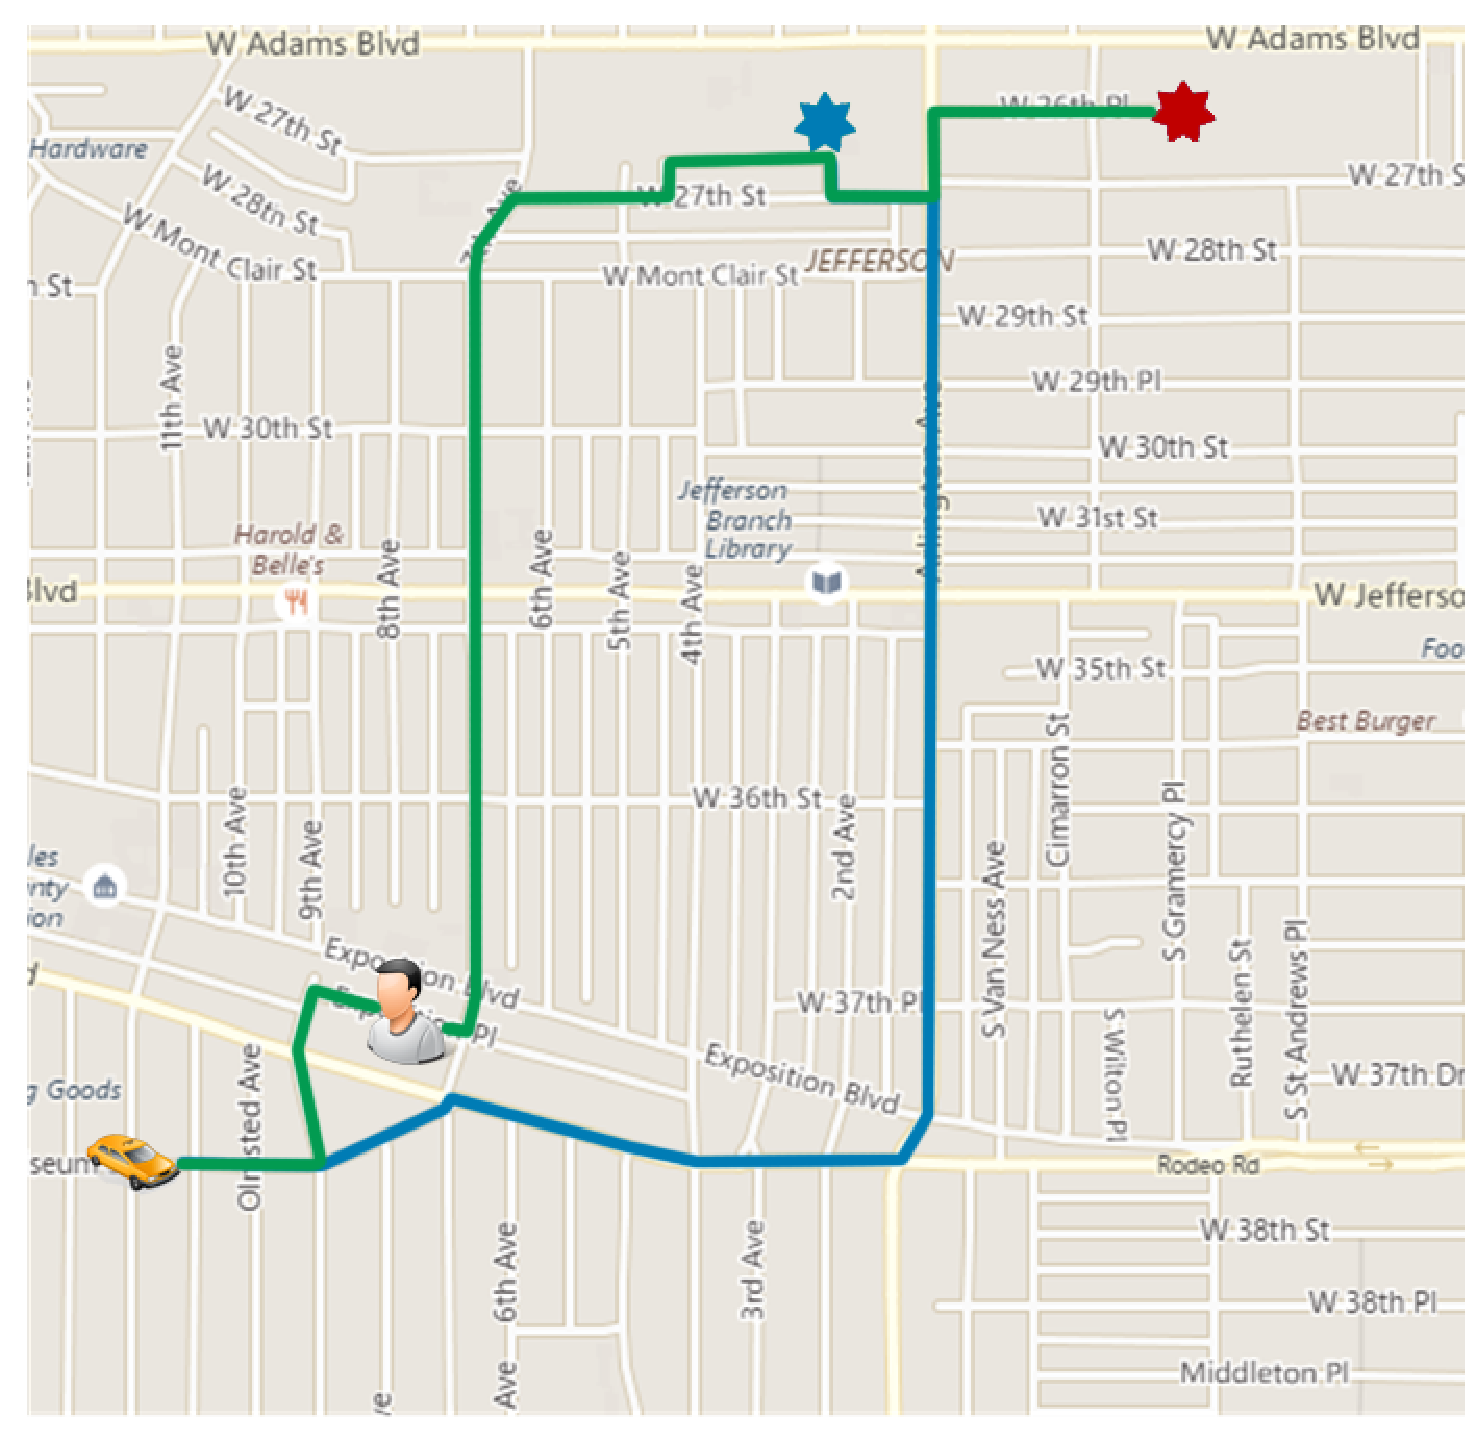
\includegraphics[width = 0.825\columnwidth]{rs_bid}
\end{figure}
}
\column{0.3\textwidth}
\only<1->{
\vspace{0.75in}
\begin{alertblock}{}
$bid = profit^* - profit$
\end{alertblock}
}
\end{columns}
\begin{equation*}
profit(\pi, \hat{\theta_d)} = \sum_{r \in \pi} fare(r) - cost(\pi, \hat{\theta_d})
\end{equation*}
\end{frame}

\section{Competitive Bidding}
\begin{frame}\frametitle{Competitive Bidding}
Every driver will attempt to maximize his own utility:
\begin{equation*}
E[u_i] = \left(v_i - s_i\left( v_i \right) \right) \cdot Prob \left[win_i\right] 
\end{equation*}
\only<1>{
\begin{itemize}
\item $Prob\left[win_1\right]$ is the probability that driver $i$ wins the auction
\item $v_i(.)$ is driver $i$'s \emph{true} valuation of the request
\item $s_i(.)$ is the \emph{strategy function} that driver $i$ applies to his true valuation to compute his optimal bid
\end{itemize}
}
\end{frame}

\begin{frame}\frametitle{Competitive Bidding}
\only<1>{
The optimal strategy function can be computed as:
\begin{equation*}
s_i^\prime\left(v_i\right) = \left(n-1\right)\left(\frac{f\left(v_i\right)\,\left(v_i - s_i\left(v_i\right)\right)}{F\left(v_i\right)}\right)
\end{equation*}
\begin{itemize}
\item $n$ is the total number of bidders\\ \textcolor{white}{Propose a Latent Space Transition Model to predict $n$}
\item $f(.)$ and $F(.)$ are the pdf and cdf of the bids\\ \textcolor{white}{We assume $f(.)$ is uniformly distributed in $[0, F(\phi_r)]$}
\end{itemize}
}
\only<2>{
The optimal strategy function can be computed as:
\begin{equation*}
s_i^\prime\left(v_i\right) = \left(n-1\right)\left(\frac{f\left(v_i\right)\,\left(v_i - s_i\left(v_i\right)\right)}{F\left(v_i\right)}\right)
\end{equation*}
\begin{itemize}
\item $n$ is the total number of bidders\\ \textcolor{red}{Propose a Latent Space Transition Model to predict $n$}
\item $f(.)$ and $F(.)$ are the pdf and cdf of the bids\\ \textcolor{white}{We assume $f(.)$ is uniformly distributed in $[0, F(\phi_r)]$}
\end{itemize}
%\begin{columns}
%\column{0.3\textwidth}
%\column{0.4\textwidth}
%\begin{block}{}
%\begin{center}
%Drivers can increase their income by 25\%
%\end{center}
%\end{block}
%\column{0.3\textwidth}
%\end{columns}
}
\end{frame}

\section{Latent Space Transition Model}
\begin{frame}\frametitle{Model}
\begin{itemize}
\item We assume we have $n$ locations
\item<2-> $\beta_p^t$ shows the number of ride requests for location $p$ at time $t$
\item<3-> $A^t$ is the \textit{network demand} matrix at time $t$:
\begin{itemize}
\item<3-> $\alpha_{pq}^t$ shows the fraction of requests at $p$ going to $q$.
\end{itemize} 
\item<4-> The number of drivers in location $p$ at time $t$:
\vspace{-0.1in}
\only<4>{
\begin{equation*}
v_p^t = \sum_{q=1}^n \alpha_{pq}^{t-1} min \left\lbrace v_q^{t-1}, \beta_q^{t-1} \right\rbrace + \delta_p^t
\end{equation*}
}
\only<5>{
\begin{equation*}
v_p^t = \sum_{q=1}^n \alpha_{pq}^{t-1} \textcolor{red}{min \left\lbrace v_q^{t-1}, \beta_q^{t-1} \right\rbrace} + \delta_p^t
\end{equation*}
}
\only<6>{
\begin{equation*}
v_p^t = \sum_{q=1}^n \alpha_{pq}^{t-1} min \left\lbrace v_q^{t-1}, \beta_q^{t-1} \right\rbrace + \textcolor{red}{\delta_p^t}
\end{equation*}
}
\only<7>{
\begin{equation*}
v_p^t = \sum_{q=1}^n \textcolor{red}{\alpha_{pq}^{t-1}} min \left\lbrace v_q^{t-1}, \beta_q^{t-1} \right\rbrace + \delta_p^t
\end{equation*}
}
\begin{itemize}
\item<5-> $min \left\lbrace v_q^{t-1}, \beta_q^{t-1} \right\rbrace$ gives the number of serviced trips at location $q$
\item<6-> $\delta_p^t$ gives the number of \textit{new} drivers entering the platform at time $t$ in location $p$ [2]
\end{itemize}
\end{itemize}
\only<6->{
\vspace{0.3in}
\tiny{[2] Cheng et. al., Where are the passengers? A grid-based gaussian mixture model for taxi bookings, SIGSPATIAL'15}
}
\end{frame}

\begin{frame}\frametitle{Latent Space Transition Model}
\begin{itemize}
\item Row $p$ in $A^t$ gives the probability distribution over destination of requests in $p$ at $t$
\begin{itemize}
\item various factors (/topics) can influence this distribution; e.g., locality, time, weather, etc.
\end{itemize}
\item<2-> We model each row of $A^t$ as a $k$ component \textit{Multinomial Mixture Model (MMM)}
\begin{itemize}
\item<3-> We assume the observed (/training) data corresponding to each row is randomly generated as follows:
\begin{enumerate}
\item We draw a latent topic $j \stackrel{iid}{\sim} \textrm{Mult}(\psi_i)$.
\item For each topic $j$, the observed data $x$ is drawn from the topic's multinomial distribution:
\begin{equation*}
x \vert j \stackrel{ind}{\sim} \textrm{Mult}(\mu_j)
\end{equation*}
\end{enumerate}
\only<4-5>{\begin{itemize}
\item<4-5> $\psi_{ij}$ is the \textbf{unknown} probability of selecting topic $j$ for row $i$
\item<5-5> $\mu_{jp}$ is the \textbf{unknown} probability of selecting location $p$ from topic $j$
\end{itemize}
}
\item<6-> We use the \textit{Maximum Log Likelihood} estimation method with the \textit{Expectation Maximization} algorithm to estimate the unknown parameters of the model.
\end{itemize}
\end{itemize}
\end{frame}

\section{SPARP Mechanism}
\frame{\frametitle{Outline}\tableofcontents[currentsection]}

\begin{frame}\frametitle{Income \& Revenue}
Assuming $\rho_r$ is the platform's share of ride $r$:
\begin{align*}
payment(\pi_d, \hat{\theta_d}) &= \sum_{r \in \pi_d} \rho_r\\
income(\pi_d, \hat{\theta_d}) &= \sum_{r \in \pi_d} fare(r) - payment(\pi_d, \hat{\theta_d})
\end{align*}
\vspace{0.2in}
\only<2->{
therefore,
\begin{equation*}
revenue(M(\mathcal{D}, \mathcal{R})) = \sum_{d \in \mathcal{D}} payments(\pi_d, \hat{\theta_d})
\end{equation*}
}
\end{frame}

\begin{frame}\frametitle{Payments}
Ideally the framework should be:
\begin{itemize}
\item Budget Balanced; i.e., $revenue(M(\mathcal{D}, \mathcal{R}) \geq 0$
\only<2->{
\begin{exampleblock}{}
If for every request $r$, $\rho_r \geq 0$, the platform is budget balanced.
\end{exampleblock}
}
\item<3-> Individually Rational; i.e., $\forall d \in \mathcal{D} \quad u(\pi_d, \hat{\theta_d}, \theta_d) \geq 0$
\only<4->{
\begin{block}{}
If for every request $r$ assigned to driver $d$, $\rho_r \leq bid_d^r$, the platform is individually rational.
\end{block}
}
\item<5-> Truthful; i.e., $\forall d \in \mathcal{D} \ \forall \hat{\theta_d} \in \Theta \quad u(\pi_d, \hat{\theta_d}, \theta_d) \leq u(\pi_d, \theta_d, \theta_d)$
\only<6->{
\begin{alertblock}{}
If for every request $r$, $\rho_r$, is set to the second highest bid, the platform is truthful.
\end{alertblock}
}
\end{itemize}
\end{frame}

\begin{frame}\frametitle{Second-price Auction}
\only<1>{
\begin{figure}
	\centering
    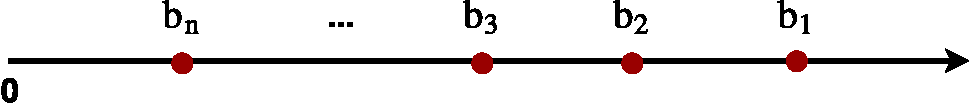
\includegraphics[width = 0.8\textwidth]{sparp1}
    \label{fig:quality}
\end{figure}
}
\only<2>{
\begin{figure}
	\centering
    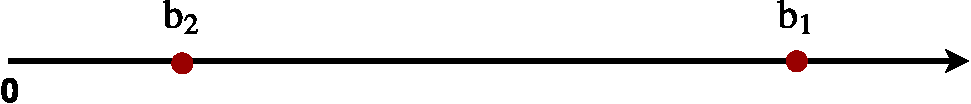
\includegraphics[width = 0.8\textwidth]{sparp2}
    \label{fig:quality}
\end{figure}
}
\only<3->{
\begin{figure}
	\centering
    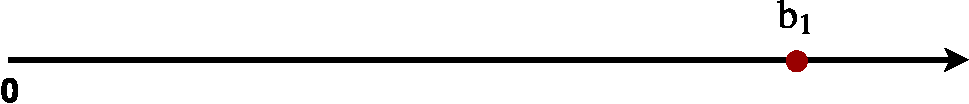
\includegraphics[width = 0.8\textwidth]{sparp3}
    \label{fig:quality}
\end{figure}
}
\begin{itemize}
\item In second-price auction, driver with $b_1$ wins but has to pay $b_2$ to the server.
\item<2-> Issues:
\begin{itemize}
\item<2-> What if $b_2$ is very small?
\item<3-> What if there is no $b_2$?
\end{itemize}
\end{itemize}
\end{frame}

\begin{frame}\frametitle{Reserved Price}
\begin{block}{}
$\forall r$, the reserved price $b_s^r$, is the minimum price the platform sets as the payment it expects. 
\end{block}
\begin{itemize}
\item<2-> If $b_s < b_2$: Driver with $b_1$ wins and pays $b_2$.
\item<3-> If $b_1 < b_s$: We assume $b_1$ wins and pays 0.
\item<4-> If $b_2 < b_s < b_1$: Driver with $b_1$ wins and pays $b_s$.
\end{itemize}
\only<4->{
\begin{figure}
	\centering
    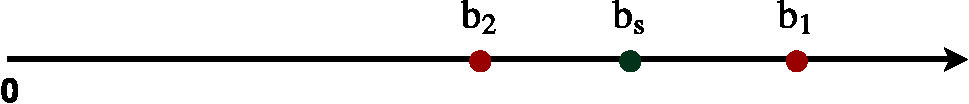
\includegraphics[width = 0.8\textwidth]{sparp4}
    \label{fig:quality}
\end{figure}
}
\only<2>{
\begin{figure}
	\centering
    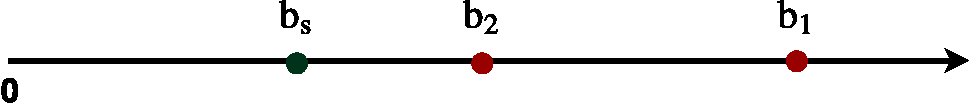
\includegraphics[width = 0.8\textwidth]{sparp5}
    \label{fig:quality}
\end{figure}
}
\only<3>{
\begin{figure}
	\centering
    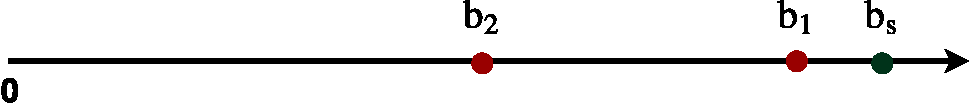
\includegraphics[width = 0.8\textwidth]{sparp6}
    \label{fig:quality}
\end{figure}
}
\begin{itemize}
\item<5-> We assume for every $r$:
\begin{columns}
\column{0.5\textwidth}
\begin{equation*}
b_s^r = F(\phi_r) - \theta^*(\phi_r)
\end{equation*}
\column{0.5\textwidth}
\vspace{-0.15in}
\begin{equation*}
\theta^* = \argmax_\theta \left\lbrace \theta(\phi_r) \mid \theta \in \Theta \right\rbrace 
\end{equation*}
\end{columns}
\end{itemize}
\end{frame}

\section{Experiments}
\frame{\frametitle{Outline}\tableofcontents[currentsection]}

\begin{frame}\frametitle{Setup}
\begin{itemize}
\item Data Set: New York City's Taxi data set
\only<1>{
\begin{itemize}
\item<1> 40K drivers \& 500K trips per day
\item<1> pickup/dropoff points, request time
\end{itemize}
}
\item<2-> Algorithms:
\only<2>{
\begin{itemize}
\item Prediction Model
\begin{itemize}
\item LSTM
\item LORE(Additive Markov Chains)[3]
\end{itemize} 
\item Revenue Generation
\begin{itemize}
\item FPACB (First-price Auction w/ Competitive Bidding)[1]
\item SPA (Second-price Auction)
\item SPARP (Second-price Auction w/ Reserved Price)
\end{itemize}
\end{itemize}
}
\item<3-> Parameters:
\only<3>{
%\vspace{-0.25in}
\begin{table}[!ht]
	\begin{center}
		\begin{tabular}{|c|c|}
			\hline
			Parameter & Values \\
			\hline \hline
            Gide Size (km) & 1, \textbf{2}, 3, 4, 5 \\ 
			\hline
			Time Slot Size (hour) & 1, \textbf{2}, 3,  4, 5, 6\\ 
			\hline
			Max Wait Time (min) & 3, \textbf{6}, 9, 12, 15, 20 \\ 
			\hline
			\# of Drivers & 1000, 2000, \textbf{5000},  10000, 20000\\ 
			\hline
			Max Passengers & 2, 3, \textbf{4}, 5, 6 \\
			\hline
			Max Allowed Detour & 25\%, \textbf{50\%}, 75\%, 100\%\\
			\hline
		\end{tabular}
	\end{center}
\end{table}
}
\item<4-> Pricing Model:
\only<4>{
\begin{equation*}
	\begin{split}
		F(\phi_r) =& 2 \times \phi_r\\
		\forall r, \lambda_r(\Delta_r) = & 1 - \Delta_r^2\\
		\forall d, \theta_d(l) = & 1.5 * l
	\end{split}
\end{equation*}
}
\end{itemize}
\only<2>{
\vspace{0.5in}
\tiny{[1] Asghari et. al., Price-aware Real-time Ride-sharing at Scale: An Auction-based Approach, SIGSPATIAL'17}\\
\tiny{[3] Zhang et. al., Lore: Exploiting sequential influence for location recommendation, SIGIR'13}
}
\end{frame}

\begin{frame}\frametitle{Prediction Model}
\begin{itemize}
\item Used k-fold cross validation to get train/test data
\item Used the Kullback-Leibler Divergence(KLD) metric to evaluate the outcome of the model:
\small{
\begin{equation*}
KLD\left(P \middle\| Q\right)=\sum_i P(i) \log \frac{P(i)}{Q(i)}
\end{equation*}
}
\end{itemize}
\vspace{-0.25in}
\begin{figure}
	\centering
    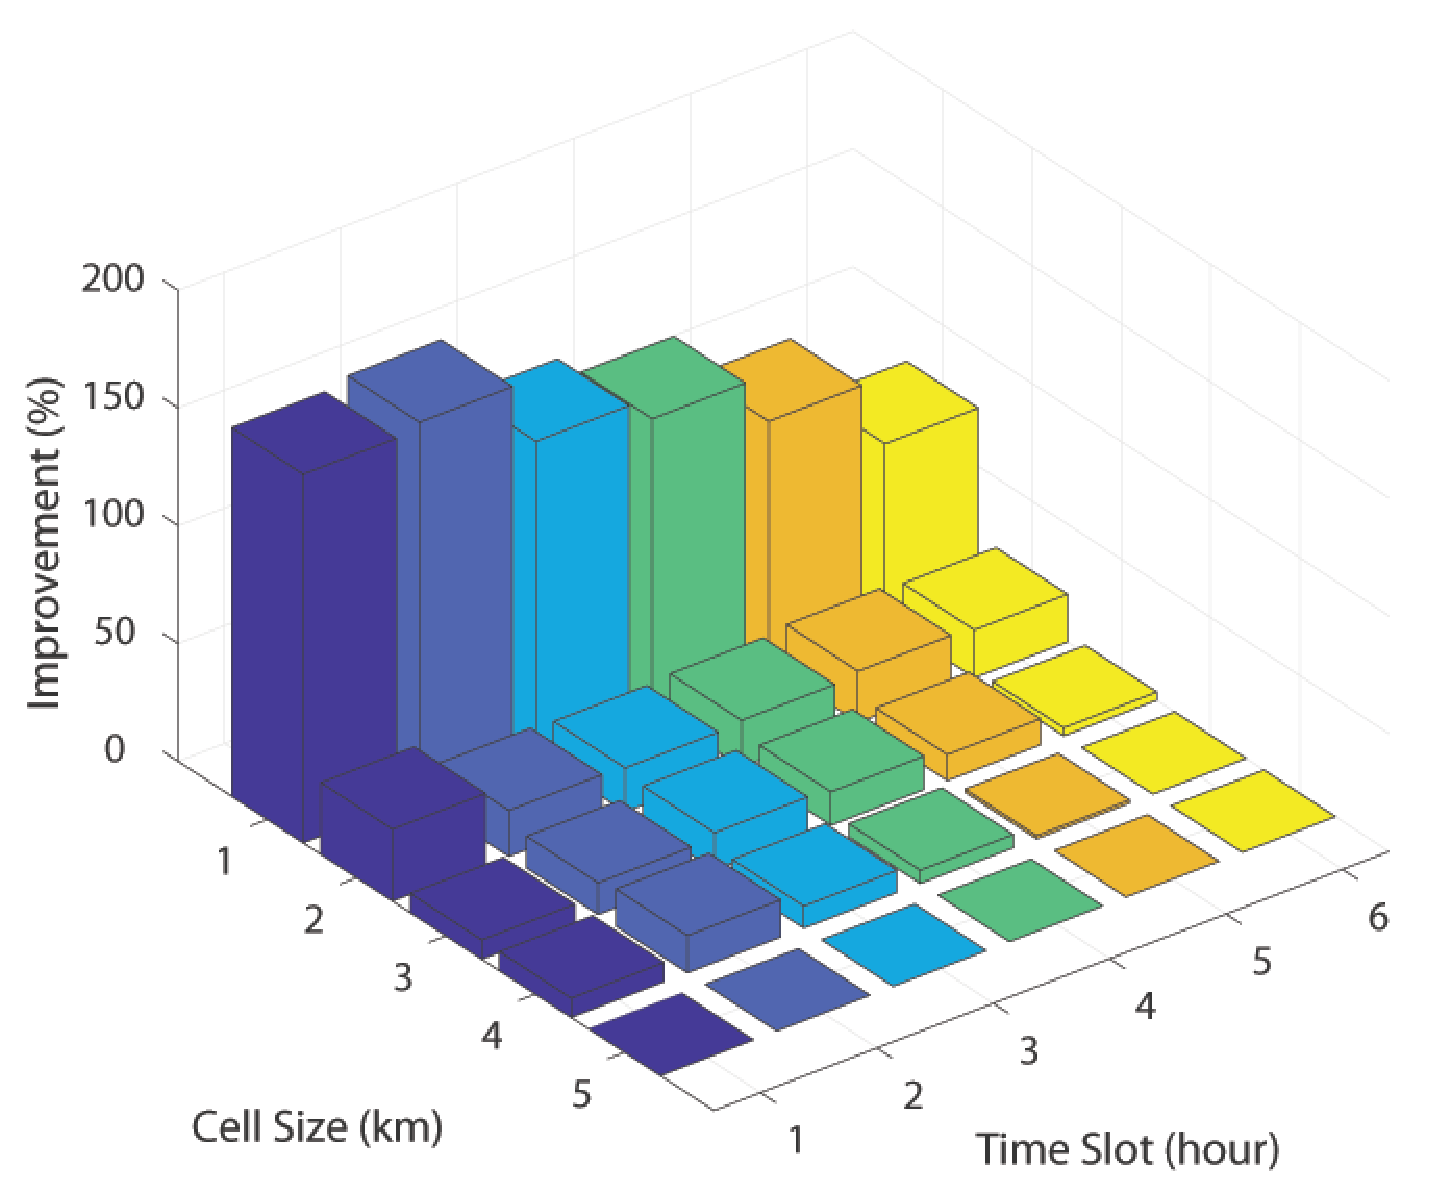
\includegraphics[width = 0.45\columnwidth]{klddiff}\\
    \tiny{\textbf{\textit{LSTM Vs LORE - Varying Cell \& Time Slot}}}
\end{figure}
\end{frame}

\begin{frame}\frametitle{Revenue Generation}
\begin{itemize}
\item Compared the revenue of SPA \& SPARP w/ that of FPACB
\end{itemize}
\begin{columns}
\column{0.5\textwidth}
\begin{figure}
	\centering
    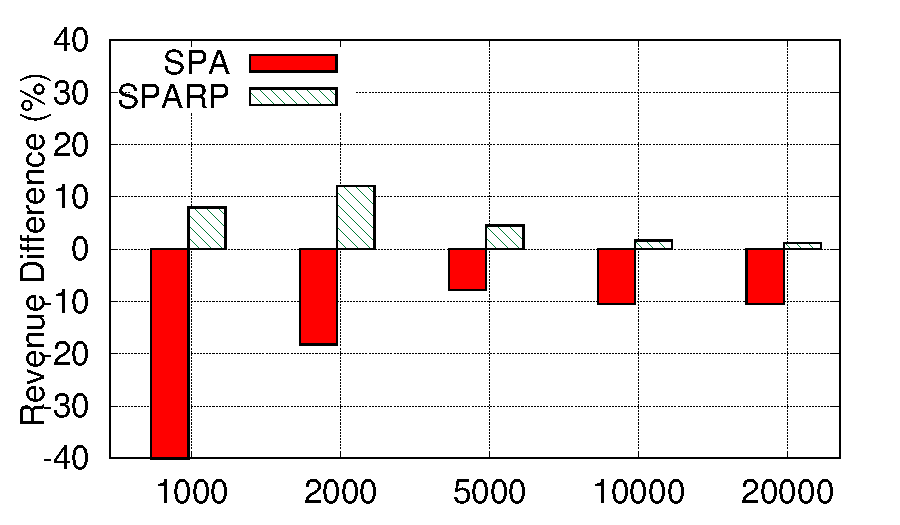
\includegraphics[width = 0.95\columnwidth]{nd2revdiff}\\
    \small{\textbf{\textit{Number of Drivers}}}
\end{figure}
\column{0.5\textwidth}
\begin{figure}
	\centering
    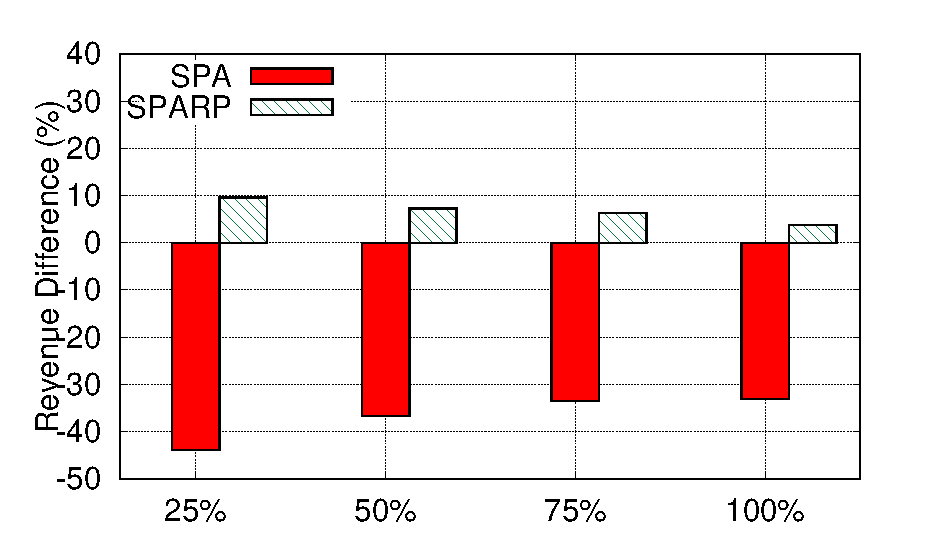
\includegraphics[width = 0.95\columnwidth]{mad2revdiff}\\
    \small{\textbf{\textit{Max Allowed Detour}}}
\end{figure}
\end{columns}
\end{frame}

\begin{frame}\frametitle{Untruthful Bidding}
\begin{itemize}
\item Use LSTM to predict the number of drivers
\item Assume the bids are uniformly distributed in $[0, F(\phi_r)]$
\end{itemize}
\begin{table}
  \centering
  \begin{tabular}{|c|c|c|c|c|}
    \hline
    \multicolumn{2}{|>{\columncolor{kugray5}}c|}{}&\multicolumn{3}{c|}{Untruthful Drivers (\%)}\\
    \arrayrulecolor{kugray5}
    \arrayrulecolor{black}
    \cline{3-5}
    \multicolumn{2}{|>{\columncolor{kugray5}}c|}{}&25\%&50\%&75\%\\
    \hline \hline
    \multirow{4}{*}{\begin{turn}{90}Trutful\end{turn}} &Assigned Requests (Average)&14.33&14.19&13.04\\
    \cline{2-5}
                         		&Assigned Requests (Median)&8&\textcolor{blue}{6}&9\\
    \cline{2-5}
                         		&Income per Mile (Average)&\$1.00&\textcolor{red}{\$1.00}&\$1.00\\
    \cline{2-5}
                         		&Income per Mile (Median)&\$1.00&\$1.00&\$1.00\\
    \hline \hline
    \multirow{4}{*}{\begin{turn}{90}Untruthful\end{turn}}&Assigned Request (Average)&13.51&13.49&12.67\\
    \cline{2-5}
                         		&Assigned Requests (Median)&7&\textcolor{blue}{6}&8\\
    \cline{2-5}
                         		&Income per Mile (Average)&\$1.24&\textcolor{red}{\$1.25}&\$1.24\\
    \cline{2-5}
                         		&Income per Mile (Median)&\$1.21&\$1.23&\$1.23\\
    \hline
  \end{tabular}
  \caption{Effects of Untruthful Bidding}
  \label{tab:untruthful}
\end{table}
\end{frame}

\section*{Q \& A}
\begin{frame}\frametitle{Questions}
\begin{center}
	
\includegraphics[scale=0.3]{QandA.jpg}
\end{center}
\end{frame}




\end{document}